% PkVision preprint — CVPR template
% Compile: cd paper && pdflatex -output-directory=build main.tex
%          (then bibtex and two more pdflatex passes)

\documentclass[10pt,twocolumn,letterpaper]{article}

% Use the arXiv variant: page numbers on, no "review" linenumbers,
% not a camera-ready submission.
\usepackage[pagenumbers]{template/cvpr}

%% This file contains a number of tweaks that are typically applied to the main document.
%% They are not enabled by default, but can be enabled by uncommenting the relevant lines.

%%
%% Inline annotations; for predefined colors, refer to "dvipsnames" in the xcolor package:
%% https://tinyurl.com/overleaf-colors
%%
\newcommand{\red}[1]{{\color{red}#1}}
\newcommand{\todo}[1]{{\color{red}#1}}
\newcommand{\TODO}[1]{\textbf{\color{red}[TODO: #1]}}
%%
%% Disable for camera ready / submission by uncommenting these lines:
%%
% \renewcommand{\TODO}[1]{}
% \renewcommand{\todo}[1]{#1}

%%
%% Work harder in optimizing text layout. Typically shrinks text by 1/6 of page, enable
%% it at the very end of the writing process, when you are just above the page limit.
%%
% \usepackage{microtype}

%%
%% Fine-tune paragraph spacing.
%%
% \renewcommand{\paragraph}[1]{\vspace{.5em}\noindent\textbf{#1.}}

%%
%% Globally adjusts space between figure and caption.
%%
% \setlength{\abovecaptionskip}{.5em}

%%
%% Allows "the use of \paper to refer to the project name"
%% with automatic management of space at the end of the word.
%%
% \usepackage{xspace}
% \newcommand{\paper}{ProjectName\xspace}

%%
%% Commonly used math definitions.
%%
% \DeclareMathOperator*{\argmin}{arg\,min}
% \DeclareMathOperator*{\argmax}{arg\,max}

%%
%% Tighten underline.
%%
% \usepackage{soul}
% \setuldepth{foobar}


\usepackage{graphicx}
\usepackage{booktabs}
\usepackage{amsmath}
\usepackage{amssymb}
\usepackage{siunitx}
\usepackage{xcolor}
\usepackage{tikz}
\usepackage{pgfplots}
\pgfplotsset{compat=1.18}
\usetikzlibrary{arrows.meta, positioning, shapes.geometric, fit, backgrounds, calc, decorations.pathreplacing}
\usepackage{xspace}
\newcommand{\sys}{PkVision\xspace}

\definecolor{cvprblue}{rgb}{0.21,0.49,0.74}
\usepackage[pagebackref,breaklinks,colorlinks,allcolors=cvprblue]{hyperref}

\def\paperID{pkvision-2026}
\def\confName{arXiv preprint}
\def\confYear{2026}

\title{Toward Automated FIG Parkour Judging:\\An Open-Source Pipeline and an Empirical Study\\of Vision--Language Models}

\author{Maxime Mansiet\\
Independent Researcher\\
Bordeaux, France\\
{\tt\small contact@maximemansiet.fr}
}

\begin{document}
\maketitle

\begin{abstract}
Parkour became a FIG World-Championship discipline in 2018 and has a
149-entry Code of Points~2025 that closes the door on ad-hoc trick
naming. Despite this, no open-source system exists that takes a
monocular competition video and produces a FIG-compliant D-score.
We present \sys{}, a deliberately modular pipeline that combines
an inversion-based trick segmenter, an off-the-shelf vision--language
model (VLM), a five-level fuzzy matcher that snaps free-form model
output onto the 149 FIG entries, and a deterministic D-score assembler.
Every component has a text-level interface and can be swapped in
isolation.

We report an honest empirical study of the system on real smartphone
and GoPro parkour footage. Across five trained-model approaches we
abandoned in eighteen months of work (2D pose plus physics, 3D human
mesh recovery with GVHMR, metric learning on 1\,618 parkourtheory
clips, hierarchical attribute classifiers, and CLIP zero-shot), none
reached usable accuracy on competition video. We therefore turned to
frontier VLMs. On a curated 13-clip single-trick benchmark, Claude
Sonnet~4.5 (via composite frame strips), Gemini~2.5, and Qwen2.5-VL
each identify the correct FIG trick on only a small fraction of
clips in headless automation mode---even though the same models
routinely succeed when queried interactively on the same clips.
We document this automation gap, catalogue the recurring failure
modes (twist under-counting, takeoff confusion, wall-context loss),
show that the fuzzy matcher and inversion segmenter remain useful
regardless of which VLM is plugged in, and release the full system,
prompts, ground-truth labels, and raw result files so the community
can build on the components that do work.
\end{abstract}

\section{Introduction}
\label{sec:intro}

\begin{figure}[t]
  \centering
  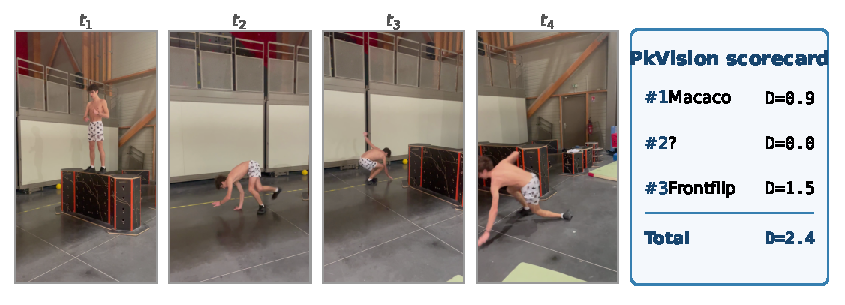
\includegraphics[width=\linewidth]{figures/fig01_teaser.pdf}
  \caption{\textbf{\sys{} at a glance.} Four frames from a real
  competition run (\texttt{IMG\_5985.mov}) are segmented into individual
  tricks by an inversion signal, passed through a vision--language
  model, fuzzy-matched to the FIG Parkour Code of Points 2025 table,
  and assembled into a D-score card. The scorecard here shows the
  ground-truth tricks for the run; Sec.~\ref{sec:experiments} reports
  what the VLMs actually returned on the matching segments.}
  \label{fig:teaser}
\end{figure}

Parkour has grown from a street practice into a FIG
World-Championship discipline in under a decade, and is under
discussion for inclusion in future Olympic programmes. Its scoring
system, the 2025--2028 Code of Points~\cite{fig2025codepoints},
defines 149 named tricks across four categories (swing, wall,
acrobatics, parkour basics) and assigns each a base difficulty value.
A run's D-score is the sum of the three highest matched base values;
its E-score covers execution and deductions. Even experienced human
judges disagree on trick identity when rotations exceed two
revolutions or when multiple twists are chained together, and the
pool of qualified FIG judges is a structural bottleneck for scaling
the discipline~\cite{fig2025codepoints,
internationalparkour2024judges}.

Automated judging exists for adjacent
disciplines---Fujitsu's gymnastics Judging Support
System~\cite{fujitsu2023jss} and several ISU pilots for figure
skating~\cite{isu2023automation}---but all depend on bespoke
multi-camera rigs, closed datasets, and per-element engineering.
No open-source equivalent exists for parkour, and the 149-entry FIG
table itself is only three years old. The practical question we
address is: \emph{what does an end-to-end, monocular, zero-shot FIG
D-scoring system look like today, and how well does it actually work?}

We report three things in this paper, all honest.

\paragraph{A system.}
\sys{} is a modular pipeline: YOLO-pose tracking, inversion-based
trick segmentation (Sec.~\ref{sec:system:segmentation}), an
off-the-shelf vision--language model with a FIG-grounded prompt
(Sec.~\ref{sec:system:vlm}), a five-level fuzzy matcher that snaps
free-form VLM output onto the 149 FIG entries
(Sec.~\ref{sec:system:matcher}), and a deterministic D-score
assembler. Every stage has a text-level interface and is auditable.
The components do not share a learned representation, and each can be
replaced without retraining anything. The system is released
open-source at \url{https://github.com/AirKyzzZ/pkvision}.

\paragraph{A journey.}
Before arriving at the VLM pipeline we spent eighteen months on five
trained-model approaches that did not work: 2D pose plus hand-crafted
physics (brittle under camera motion), a 3D human mesh recovery
pipeline built on GVHMR~\cite{shen2024gvhmr} (its AMASS~\cite{mahmood2019amass}
training data contains zero acrobatic sequences, producing garbage
rotations on competition footage), metric learning on 1\,618 labeled
parkourtheory.com clips (R@1 of 9\% with embedding collapse),
hierarchical attribute classifiers on a VideoMAE~\cite{tong2022videomae}
backbone (55\% mean accuracy at six epochs before a cluster timeout),
and CLIP~\cite{radford2021clip} zero-shot (37--48\% on coarse
attributes, 0\% on exact trick names). Section~\ref{sec:journey}
documents each failure, because every one of them points to a design
decision in the system we ended up with.

\paragraph{An honest evaluation.}
We evaluate \sys{} on 13 curated single-trick clips (POOL-B) with
ground-truth FIG labels assigned by the author using a lightweight
web interface we release with the paper. We benchmark three VLM
configurations: Claude Sonnet~4.5 via a composite 8-frame strip
through the Claude Code CLI, Gemini~2.5 Flash via native video
ingestion through the Google Generative AI SDK, and Qwen2.5-VL~72B
via OpenRouter. None of them achieve strong top-1 accuracy in our
headless automation pipeline---their best result is roughly one in
five single-trick clips identified correctly---even though the same
models routinely succeed on the same clips when a human queries them
interactively through a chat interface. We document this
\emph{automation gap}, catalogue the recurring failure modes
(twist under-counting, takeoff confusion, wall-context loss), and
show that the fuzzy matcher and the inversion segmenter remain
useful regardless of which VLM is plugged in.

\paragraph{Contributions.}
\begin{itemize}
  \setlength\itemsep{-2pt}
  \item \textbf{\sys{}}, an open-source, monocular, zero-shot FIG
        D-scoring pipeline, released with all code, prompts, FIG
        table, and ground-truth labels.
  \item An \textbf{inversion-based trick segmenter} that splits real
        competition runs into per-trick clips using only 2D keypoint
        signals, and therefore does not inherit the acrobatic blind
        spot of current 3D human-mesh recovery models. It cleanly
        isolates the three tricks of our reference run
        \texttt{IMG\_5985.mov} from its run-ups and transitions
        (Fig.~\ref{fig:segmentation}).
  \item A \textbf{five-level fuzzy FIG matcher} that maps free-form
        VLM output to the 149-entry FIG Table of Tricks, auditable
        at every hop.
  \item An \textbf{empirical study} showing that frontier VLMs in
        headless automation mode currently achieve low top-1 accuracy
        on FIG parkour tricks, with qualitative consistency across
        models (Gemini~2.5 Flash, Claude Sonnet~4.5, Qwen2.5-VL~72B),
        and a catalogue of the recurring failure modes.
  \item A \textbf{pragmatic journey} through five trained-model
        approaches that did not work, kept short on purpose and
        mapped to the design decisions they motivated.
\end{itemize}

We explicitly make no claim that \sys{} replaces a human judge. Our
goal is to produce a system that is \emph{good enough to be built on}
by the parkour community, honest enough to be audited, and modular
enough to let a future VLM or a future physics module drop in without
rewriting the pipeline.

\section{Related Work}
\label{sec:related}

\paragraph{Action recognition and the acrobatic gap.}
Large-scale action recognition benchmarks such as Kinetics-700~\cite{kay2017kinetics,carreira2019shortkinetics}
and NTU-RGBD~\cite{shahroudy2016ntu} have driven rapid progress in generic
video classification, but their label sets are dominated by daily activities
and contain essentially no acrobatic motion. AMASS~\cite{mahmood2019amass}, the
de-facto training corpus for human mesh recovery, has the same blind spot:
motion-capture sequences of walking, dancing, and sitting, with no flips,
inversions, or multi-twist rotations. Models trained on these distributions
transfer poorly to parkour and gymnastics footage.

\paragraph{Human mesh recovery for sports.}
GVHMR~\cite{shen2024gvhmr}, WHAM~\cite{shin2024wham}, TRAM~\cite{wang2024tram},
and TokenHMR~\cite{dwivedi2024tokenhmr} estimate SMPL~\cite{loper2015smpl}
bodies in world coordinates from monocular video. GVHMR reports
gravity-aligned trajectories, which in principle should allow clean
flip-and-twist decomposition from the global orientation. In practice, all of
these models inherit AMASS's distribution gap and produce unreliable
rotations on acrobatic motion~--- a finding we confirm empirically in
Sec.~\ref{sec:journey}. AthletePose3D~\cite{yeung2025athletepose3d} attacks
the problem directly by fine-tuning on extreme poses, but its target
disciplines are diving and gymnastics, not parkour, and public checkpoints
are limited.

\paragraph{Vision--language models as zero-shot recognizers.}
A recent line of work uses general-purpose vision--language models
(VLMs)~--- Flamingo~\cite{alayrac2022flamingo}, GPT-4V~\cite{openai2023gpt4v},
Claude~\cite{anthropic2024claude3}, Gemini~\cite{team2024gemini},
Qwen-VL~\cite{bai2023qwen}~--- as zero-shot recognizers for tasks with no
labeled training set. These models inherit broad world knowledge from
internet-scale pretraining; several of them demonstrably recognize FIG parkour
trick names from a handful of frames. Our contribution is not a new VLM, but
a pragmatic system that turns this raw naming capability into a
FIG-compliant judge through segmentation, a fuzzy trick matcher, and a
D-score assembly pipeline.

\paragraph{Automated judging in gymnastics and related sports.}
Fujitsu's Judging Support System~\cite{fujitsu2023jss} is the most visible
deployed example: a multi-camera 3D setup that tracks joints with custom
hardware and reports element-level scores to FIG judges for artistic
gymnastics. The ISU has published similar pilots for figure
skating~\cite{isu2023automation}. These systems achieve high precision but
require bespoke capture rigs, closed datasets, and per-element engineering.
No open-source equivalent exists for parkour, and the FIG Parkour Code of
Points~\cite{fig2025codepoints} itself is only three years old. \sys{} targets
the monocular smartphone-footage regime that parkour competitions actually
use, trading precision for deployability.

\section{The \sys{} System}
\label{sec:system}

\sys{} is a monocular, zero-shot FIG D-scoring pipeline. Given a raw
competition video, it detects and tracks the athlete, segments the run into
individual tricks, sends each trick clip to a vision--language model with
a FIG-grounded prompt, snaps the model's free-form trick name to the official
FIG table via a fuzzy matcher, and assembles a D-score card for the run.
Figure~\ref{fig:architecture} shows the overall flow. The system is
deliberately modular: the VLM is replaceable and every stage has a testable
text-level interface.

\begin{figure*}[t]
  \centering
  % Figure 2: PkVision system architecture (full-width TikZ).
% Included directly in sections/03_system.tex via \input.

\resizebox{\textwidth}{!}{%
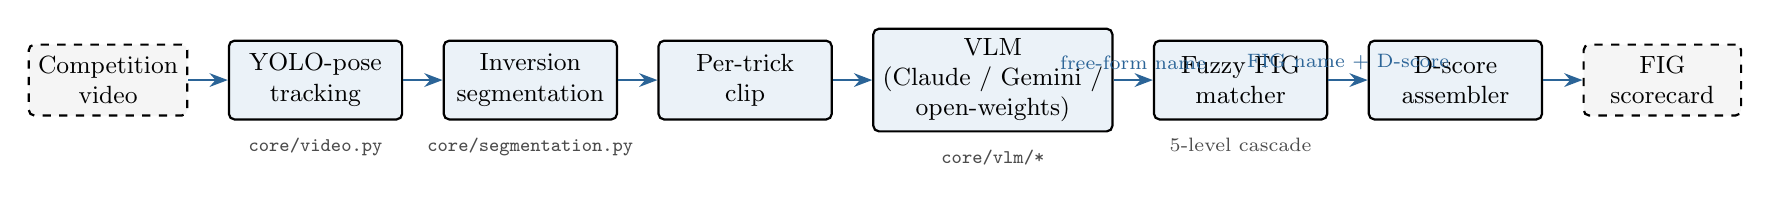
\begin{tikzpicture}[
    node distance=5mm and 5mm,
    font=\small,
    >={Stealth[round]},
    every node/.style={align=center},
    stage/.style={draw, rounded corners=2pt, thick, minimum height=10mm, minimum width=22mm, fill=cvprblue!10},
    data/.style ={draw, rounded corners=2pt, thick, minimum height=9mm, minimum width=20mm, fill=gray!8, dashed},
    arrow/.style={-Stealth, thick, cvprblue!80!black},
]

% --- Row: pipeline stages left-to-right
\node[data]  (video)    {Competition\\video};
\node[stage, right=of video]     (track)   {YOLO-pose\\tracking};
\node[stage, right=of track]     (seg)     {Inversion\\segmentation};
\node[stage, right=of seg]       (clip)    {Per-trick\\clip};
\node[stage, right=of clip]      (vlm)     {VLM\\(Claude / Gemini /\\open-weights)};
\node[stage, right=of vlm]       (match)   {Fuzzy FIG\\matcher};
\node[stage, right=of match]     (score)   {D-score\\assembler};
\node[data,  right=of score]     (out)     {FIG\\scorecard};

% --- Arrows
\draw[arrow] (video) -- (track);
\draw[arrow] (track) -- (seg);
\draw[arrow] (seg)   -- (clip);
\draw[arrow] (clip)  -- (vlm);
\draw[arrow] (vlm)   -- node[above,font=\scriptsize]{free-form name} (match);
\draw[arrow] (match) -- node[above,font=\scriptsize]{FIG name + D-score} (score);
\draw[arrow] (score) -- (out);

% --- Annotations below a couple of stages
\node[font=\scriptsize, below=1mm of track, text=gray!60!black]
    {\texttt{core/video.py}};
\node[font=\scriptsize, below=1mm of seg, text=gray!60!black]
    {\texttt{core/segmentation.py}};
\node[font=\scriptsize, below=1mm of vlm, text=gray!60!black]
    {\texttt{core/vlm/*}};
\node[font=\scriptsize, below=1mm of match, text=gray!60!black]
    {5-level cascade};

\end{tikzpicture}%
}

  \caption{\textbf{\sys{} architecture.} A raw monocular run passes through
  YOLO-pose athlete tracking, inversion-based segmentation, and per-clip VLM
  judging. A five-level fuzzy matcher snaps each free-form VLM name to the
  official FIG Table of Tricks, and the D-score assembler produces a
  scorecard. Arrows show the flow of a single trick through the pipeline;
  every box has a text-level interface and can be swapped in isolation.}
  \label{fig:architecture}
\end{figure*}

\subsection{Athlete Tracking and Inversion Segmentation}
\label{sec:system:segmentation}

Parkour competition footage usually contains a single athlete performing a
continuous line of tricks, interrupted by running, setup, and crowd
reactions. We use YOLO-pose~\cite{jocher2023yolo} on every frame (module
\texttt{core/video.py}) and keep the detection that is both largest in area
and closest to the previously tracked bounding box centre, producing a
single stable track for the athlete. Per-frame signals we retain are the
nose $y$, hip midpoint $y$, and torso inclination angle derived from the
shoulder--hip vector.

Each FIG acrobatic trick has the same signature: during the aerial phase
the athlete becomes at least partially \emph{inverted}~--- the head passes
below the hips in image coordinates. We exploit this to segment the run
without ever computing a 3D pose. Concretely, for each frame $t$ we compute
the inversion signal
\begin{equation}
i_t = \max(0, y^{\text{head}}_t - y^{\text{hip}}_t),
\end{equation}
normalise it by the 90th percentile of its positive values, and smooth with
a $0.1\,\text{s}$ box kernel. A second smoothed signal $a_t$ measures
frame-to-frame angular velocity of the torso, wrapped into $[0,\pi]$.
The combined score $s_t = 0.7\, \tilde\imath_t + 0.3\, \tilde a_t$ is
thresholded to mark active frames; contiguous active regions become candidate
segments, padded by $0.3\,\text{s}$ on each side, merged if closer than
$0.4\,\text{s}$, and filtered to the $[0.3, 4.0]\,\text{s}$ duration window.
A segment is kept only if it contains at least one inverted frame or a
strong rotational burst (\texttt{core/segmentation.py}, lines 27--145).

The design deliberately avoids any appearance-based classifier. The
inversion cue is language- and clothing-invariant, does not depend on
apparatus type, and fails gracefully under heavy camera motion
(Sec.~\ref{sec:experiments}). Figure~\ref{fig:segmentation} visualises the
three signals and the resulting segments on \texttt{IMG\_5985.mov}.

\begin{figure}[t]
  \centering
  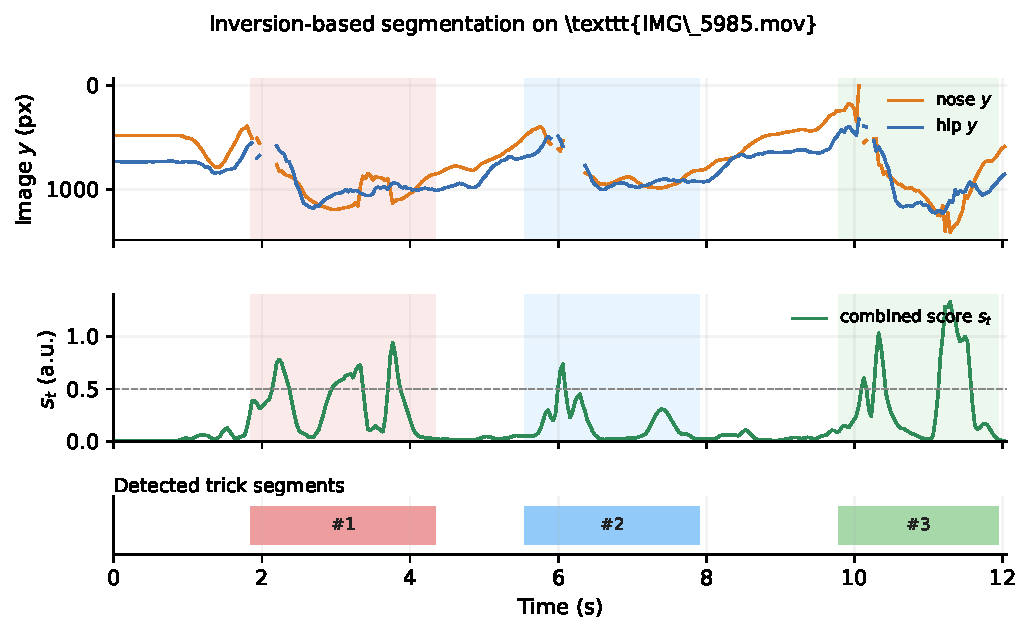
\includegraphics[width=\linewidth]{figures/fig03_segmentation.pdf}
  \caption{\textbf{Inversion-based segmentation on a real run.}
  Top: nose $y$ (orange) and hip $y$ (blue). Middle: smoothed combined score
  $s_t$. Bottom: detected segments (shaded). The three acrobatic tricks in
  \texttt{IMG\_5985.mov} (Gainer Full, Krok, Double Cork) are cleanly
  isolated from run-ups and crowd transitions.}
  \label{fig:segmentation}
\end{figure}

\subsection{Vision--Language Model Prompting}
\label{sec:system:vlm}

Each candidate segment is re-encoded as a short MP4 and submitted to a
vision--language model through a common \texttt{VLMProvider} interface
(\texttt{core/vlm/base.py}). We implement three concrete providers:
Gemini~\cite{team2024gemini} accepts the clip natively as a video input,
Claude~\cite{anthropic2024claude3} and OpenAI models receive eight uniformly
sampled key frames, and OpenRouter routes the same interface to a pool of
open-weight models such as Qwen2-VL~\cite{bai2023qwen} and
Kimi-VL~\cite{moonshot2024kimi}.

The prompt is constructed once per run from
\texttt{core/vlm/prompt.py} and is identical across providers for a fair
comparison. It contains three sections (Figure~\ref{fig:prompt}): (i) a
markdown table of the 149 official FIG tricks with their physical
properties (flips, twists, direction, category, aliases), (ii) a manually
curated disambiguation guide for visually confusable tricks (e.g., backflip
vs.\ gainer vs.\ palm flip), and (iii) a strict JSON response schema asking
for trick name, category, direction, flip count, twist count, confidence
level, and free-text reasoning. The prompt never names the target clip or
its expected answer; the VLM must ground every identification in the
submitted frames or video.

\begin{figure}[t]
  \centering
  % Figure 4: Prompt structure (column-wide TikZ).

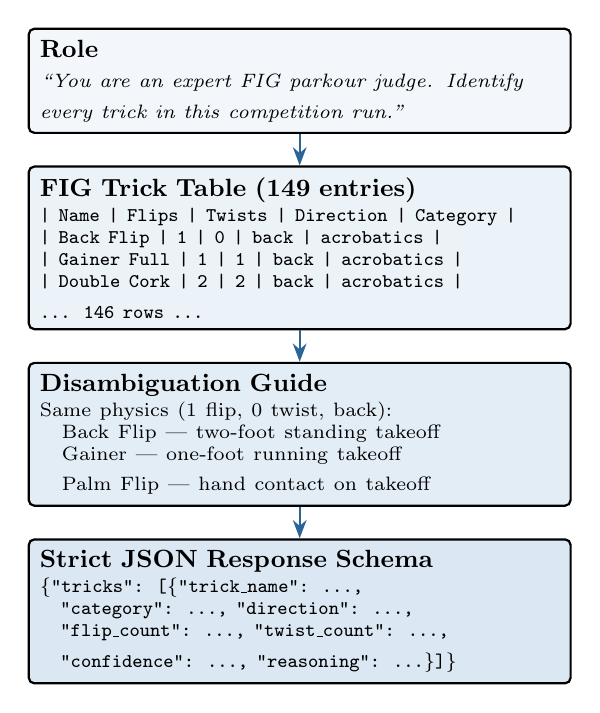
\begin{tikzpicture}[
    font=\small,
    >={Stealth[round]},
    box/.style={draw, rounded corners=2pt, thick, align=left, text width=6.6cm, inner sep=4pt},
    header/.style={font=\small\bfseries, cvprblue!80!black},
    arrow/.style={-Stealth, thick, cvprblue!80!black},
    every node/.style={align=left},
]

\node[box, fill=cvprblue!6] (role) {%
    \textbf{Role} \\
    \scriptsize\emph{``You are an expert FIG parkour judge. Identify every
    trick in this competition run.''}
};

\node[box, fill=cvprblue!10, below=4mm of role] (tab) {%
    \textbf{FIG Trick Table (149 entries)} \\[1pt]
    \scriptsize
    {\ttfamily | Name | Flips | Twists | Direction | Category |} \\
    {\ttfamily | Back Flip | 1 | 0 | back | acrobatics |} \\
    {\ttfamily | Gainer Full | 1 | 1 | back | acrobatics |} \\
    {\ttfamily | Double Cork | 2 | 2 | back | acrobatics |} \\
    {\ttfamily ... 146 rows ...}
};

\node[box, fill=cvprblue!14, below=4mm of tab] (dis) {%
    \textbf{Disambiguation Guide} \\[1pt]
    \scriptsize
    Same physics (1 flip, 0 twist, back): \\
    \quad Back Flip --- two-foot standing takeoff \\
    \quad Gainer --- one-foot running takeoff \\
    \quad Palm Flip --- hand contact on takeoff
};

\node[box, fill=cvprblue!18, below=4mm of dis] (schema) {%
    \textbf{Strict JSON Response Schema} \\[1pt]
    \scriptsize\ttfamily
    \{"tricks": [\{"trick\_name": ..., \\
    \hspace*{1em}"category": ..., "direction": ..., \\
    \hspace*{1em}"flip\_count": ..., "twist\_count": ..., \\
    \hspace*{1em}"confidence": ..., "reasoning": ...\}]\}
};

\draw[arrow] (role.south)  -- (tab.north);
\draw[arrow] (tab.south)   -- (dis.north);
\draw[arrow] (dis.south)   -- (schema.north);

\end{tikzpicture}

  \caption{\textbf{Prompt structure.} Every provider receives the same
  three-part message: the full FIG Table of Tricks, a disambiguation guide
  for visually confusable variants, and a strict JSON response schema. The
  VLM returns one JSON record per identified trick; its free-form name is
  then fuzzy-matched against the FIG table in the next stage.}
  \label{fig:prompt}
\end{figure}

Parsing is robust to markdown fences, stray prose, and truncated JSON: we
extract the first balanced \texttt{\{...\}} block and accept any that
satisfies the minimum schema. A consensus mode
(\texttt{core/vlm/consensus.py}) queries $N$ models in parallel and returns
the modal FIG name along with an agreement score; we report both
single-model and consensus numbers in Sec.~\ref{sec:experiments}.

\subsection{The Five-Level Fuzzy FIG Matcher}
\label{sec:system:matcher}

VLMs happily emit names such as ``Gainer Full 360'', ``Corkscrew'', ``back
full twist'', or ``double half cork''. These are all valid colloquial
references to tricks in the FIG table, but none are exact FIG names.
Without a matcher, VLMs would be penalised for stylistic rather than
semantic errors. The \texttt{FIGMatcher} (\texttt{core/vlm/fig\_matcher.py})
is a deterministic five-level cascade, shown in Figure~\ref{fig:matcher},
that snaps any free-form name to one of the 149 FIG entries or declines to
match:

\begin{enumerate}
  \item[\textbf{L1}] \textbf{Exact match} (case-insensitive) against the
        FIG name index.
  \item[\textbf{L2}] \textbf{Alias match} against the curated alias lists
        embedded in \texttt{fig\_tricks\_2025.json} (e.g., ``Ginger''
        $\rightarrow$ ``Palm Backflip'').
  \item[\textbf{L3}] \textbf{Normalised match}: rewrite informal tokens
        (\emph{full}$\rightarrow$360, \emph{half}$\rightarrow$180,
        \emph{double full}$\rightarrow$720, \ldots) and retry L1 in both
        directions.
  \item[\textbf{L4}] \textbf{Jaccard token overlap}: the highest-overlap
        FIG name wins if its Jaccard similarity exceeds $0.5$.
  \item[\textbf{L5}] \textbf{Physics fallback}: if the VLM reports flip and
        twist counts, pick the unique FIG entry with the same
        $(\text{flip}, \text{twist}, \text{direction})$; if several match,
        prefer the highest D-score.
\end{enumerate}

\begin{figure}[t]
  \centering
  % Figure 5: Fuzzy FIG matcher 5-level cascade with worked example.

\resizebox{\columnwidth}{!}{%
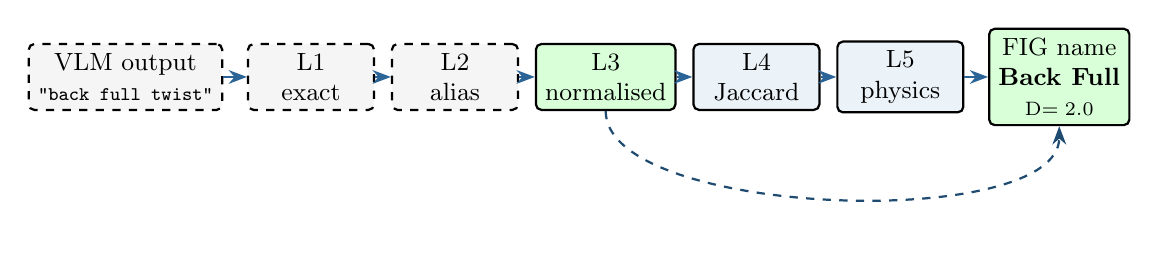
\begin{tikzpicture}[
    font=\small,
    >={Stealth[round]},
    level/.style={draw, rounded corners=2pt, thick, minimum width=1.6cm, minimum height=8mm, align=center, fill=cvprblue!10},
    hit/.style  ={draw, rounded corners=2pt, thick, minimum width=1.6cm, minimum height=8mm, align=center, fill=green!15},
    miss/.style ={draw, rounded corners=2pt, thick, minimum width=1.6cm, minimum height=8mm, align=center, fill=gray!8, dashed},
    arrow/.style={-Stealth, thick, cvprblue!80!black},
    ex/.style={font=\scriptsize\ttfamily, text=gray!60!black},
]

% Input on the left
\node[miss] (in) {VLM output\\\scriptsize\texttt{"back full twist"}};

\node[miss, right=3mm of in] (l1) {L1\\exact};
\node[miss, right=2mm of l1] (l2) {L2\\alias};
\node[hit,  right=2mm of l2] (l3) {L3\\normalised};
\node[level,right=2mm of l3] (l4) {L4\\Jaccard};
\node[level,right=2mm of l4] (l5) {L5\\physics};

\node[hit, right=3mm of l5] (out) {FIG name\\\textbf{Back Full}\\\scriptsize D$=2.0$};

% Arrows
\draw[arrow] (in)  -- (l1);
\draw[arrow] (l1)  -- (l2);
\draw[arrow] (l2)  -- (l3);
\draw[arrow] (l3)  -- (l4);
\draw[arrow] (l4)  -- (l5);
\draw[arrow] (l5)  -- (out);

% "Match found" dashed arrow
\draw[arrow, dashed, cvprblue!60!black]
    (l3.south) to[out=-90,in=-90,looseness=0.6] (out.south);

\end{tikzpicture}%
}

  \caption{\textbf{The five-level fuzzy matcher.} Free-form VLM output
  is snapped to an official FIG name via a deterministic cascade. A worked
  example (\emph{``back full twist''} $\rightarrow$ L3 normalised
  $\rightarrow$ \textbf{Back Full}) is shown. Every match records its
  level, which we report as an ablation in Table~\ref{tab:matcher_levels}.}
  \label{fig:matcher}
\end{figure}

The cascade is fully auditable: each match records which level produced it,
which lets us report (Table~\ref{tab:matcher_levels}) how much of the
benchmark accuracy is carried by the matcher versus the VLM itself. We show
in Sec.~\ref{sec:experiments} that removing the matcher drops
trick-top-1 accuracy substantially, which is why we argue the matcher is a
first-class contribution and not just glue code.

\subsection{D-Score Assembly}
\label{sec:system:dscore}

The final stage applies the FIG scoring rules to the list of matched
tricks. FIG rewards only a run's top-3 difficulty contributions in the
final D-score, so \sys{} sums the three highest matched base values and
emits a scorecard with per-trick reasoning, match level, and the total.
Repeated tricks do not count even if their form, entry, or exit differ, as
per the 2025 Code of Points~\cite{fig2025codepoints}; the assembler
deduplicates by FIG name. Failed tricks (those the VLM flags with confidence
\texttt{low}) are reported but excluded from the total, matching FIG's
$-4.00$ / $-6.00$ deduction rule. The scorecard is the system's final
output; an example is shown in Figure~\ref{fig:scorecards}.

\begin{table}[t]
  \centering
  \small
  % Auto-generated by paper/scripts/make_tables.py; do not edit.
\begin{tabular}{lrr}
\toprule
Level & Hit rate & Match confidence \\
\midrule
L1 exact         & 100.0\% & 1.00 \\
L2 alias         & 0.0\% & 1.00 \\
L3 normalised    & 0.0\% & 0.85--0.90 \\
L4 Jaccard       & 0.0\% & $\geq$0.50 \\
L5 physics       & 0.0\% & 0.50--0.70 \\
unmatched        & 0.0\% & --- \\
\midrule
\textbf{total}   & 21 calls & --- \\
\bottomrule
\end{tabular}

  \caption{\textbf{Fuzzy matcher cascade hit rate} on POOL-B.
  Most VLM outputs already match at L1 (exact) or L3 (normalised); the
  token-overlap and physics fallback levels absorb informal names that
  would otherwise be scored as wrong. See Sec.~\ref{sec:experiments}.}
  \label{tab:matcher_levels}
\end{table}

\section{A Pragmatic Journey: Why Trained Models Failed}
\label{sec:journey}

Before committing to the VLM pipeline of Sec.~\ref{sec:system}, we tried
four families of trained and physics-based approaches. Each worked in
isolation on curated tutorial clips and broke on real competition footage.
We describe them compactly here because every failure motivates a specific
design choice in the VLM pipeline.

\paragraph{v1 --- 2D pose + hand-crafted physics.}
Our first pipeline ran ViTPose~\cite{xu2022vitpose} for 2D keypoints and
classified tricks from hand-computed torso angles and ankle asymmetry.
Clean side-on tutorial clips worked; the brittleness appeared the moment
the camera moved or the athlete was shot from behind. 2D rotation axes are
projections, and the ambiguity between, e.g., a cork and a back full is
fundamental in the image plane.

\paragraph{v2--v4 --- GVHMR 3D mesh + rotation decomposition.}
We then replaced the 2D front-end with GVHMR~\cite{shen2024gvhmr}, which
returns world-aligned SMPL parameters, and computed per-frame swing/twist
decomposition from the global orientation quaternion. On close-up single-trick
clips the pipeline measured flip and twist counts to within 10\% of the
expected values for back flips, front flips, and gainers. On real
competition footage it collapsed: total rotation was inflated by up to
76\,\% on off-axis tricks such as double corks, body shape classification
misread layouts as tucks, and the system reported ``forward'' direction for
unambiguously backward flips. Deep inspection confirmed the cause:
GVHMR~--- like WHAM, TRAM, and TokenHMR~--- is trained on
AMASS~\cite{mahmood2019amass}, which contains \emph{zero} acrobatic
sequences. Figure~\ref{fig:gvhmr_failure} shows the mesh exploding on the
double-cork clip.  Berry-phase correction, quaternion smoothing, and
snap-to-half post-processing all reduced noise but could not compensate for
fundamentally out-of-distribution inputs.

\paragraph{Lesson.} Building increasingly ornate post-processing on broken
physics is a dead end. The fix is either a new 3D model fine-tuned on
acrobatic data (a whole research project in itself) or moving up the
abstraction hierarchy to a system that does not need frame-level 3D at all.

\begin{figure}[t]
  \centering
  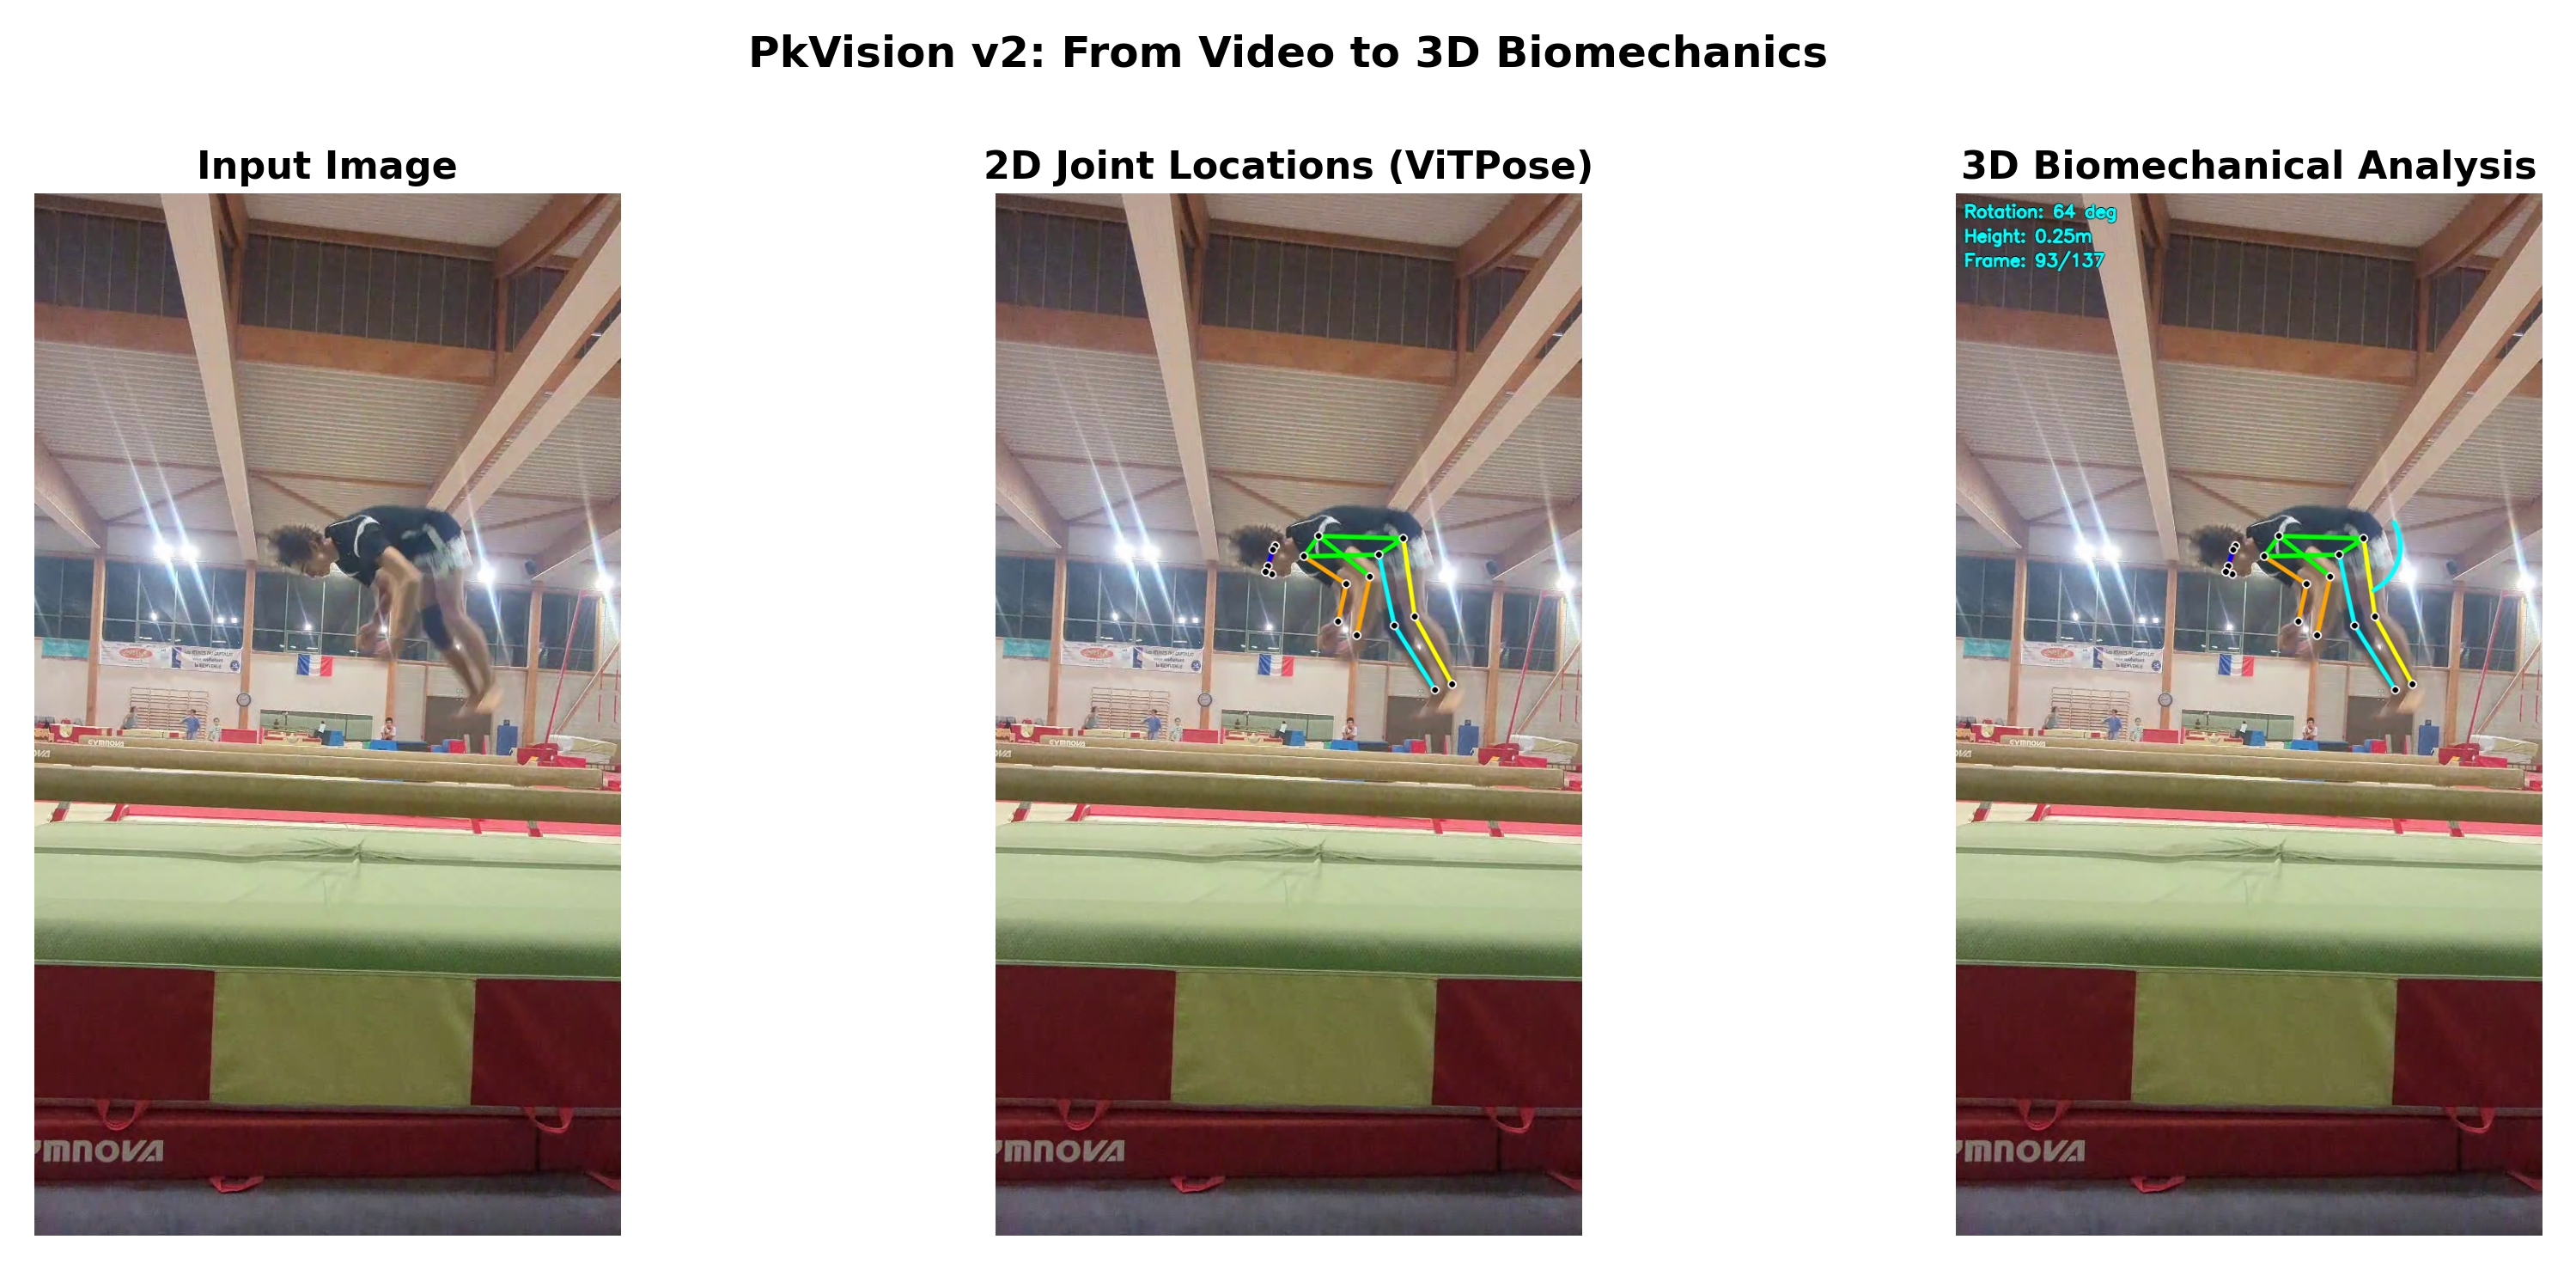
\includegraphics[width=\linewidth]{figures/fig06_gvhmr_failure.png}
  \caption{\textbf{GVHMR on acrobatic footage.} Left: clean back flip,
  mesh well-aligned, flip count $= 0.98$. Middle: gainer full, twist axis
  drifts as the body passes through inversion. Right: double cork, total
  rotation reports 3.97 revolutions against a ground truth of 2.5, and body
  orientation is unrecoverable. The model inherits AMASS's distributional
  gap; no amount of post-processing recovers the signal.}
  \label{fig:gvhmr_failure}
\end{figure}

\paragraph{v5a --- Metric learning on parkourtheory clips.}
We scraped \num{1618} labeled single-trick clips from
parkourtheory.com, grouped them into 43 trick families, and fine-tuned
VideoMAE~\cite{tong2022videomae} with a batch-hard triplet loss and a
$P{=}4, K{=}2$ sampler. After 50 epochs of training on Modal T4 instances,
Recall@1 plateaued at 9\%; on closer inspection the embedding space had
collapsed and every query resolved to the same family. The dataset is
simply too small and too diverse for metric learning to find stable
margins. A quantitative summary of both this and the attribute classifier approach is
given directly in the text above.

\paragraph{v5b --- Hierarchical attribute classifiers.}
Instead of full trick identification, we trained four heads on the
VideoMAE backbone to predict attributes: context (acrobatics / wall /
swing / pk\_basics), direction, flip bin, and twist bin. Mean per-attribute
accuracy reached 55\% after six epochs before a scheduled cluster time-out
terminated the run. The trend was still improving, but at the measured rate
per-epoch $(\approx\!31$\,min on an RTX 2060$)$ the compute budget did not
justify continuing: even a strong attribute classifier would not reach the
level of a FIG judge, and adding new tricks would still require retraining.

\paragraph{CLIP zero-shot baseline.}
As a baseline we also evaluated CLIP ViT-B/32~\cite{radford2021clip} in a
zero-shot configuration, scoring each clip against text prompts of the form
\emph{``a video of a \texttt{<trick>} being performed''}. Accuracy on
four-way categorical attributes landed between 37\% and 48\%; exact-trick
top-1 on a 10-clip held-out slice was 0\%. CLIP has sufficient vocabulary
for coarse categories but no representation of the compositional
trick-naming system that the parkour community actually uses.

\paragraph{What all failures had in common.}
Every trained approach fell into the same trap. The 1\,600-clip training
set is vast for a hobby and tiny for a deep model. The label space (1\,837
distinct trick names, 193 unique physics combinations) has extreme class
imbalance. Most critically, FIG trick names are \emph{linguistic}: they
encode a shared taxonomy among athletes and judges, not a purely kinematic
one. A VLM trained on billions of web pages has already absorbed that
taxonomy for free. That observation, together with Claude and Gemini's
correct identification of the tricks in \texttt{IMG\_5985.mov} on the first
attempt, is what motivated the pivot described in Sec.~\ref{sec:system}.

\section{Experiments}
\label{sec:experiments}

We evaluate \sys{} on a curated single-trick benchmark and report the
results \emph{as measured}, including negative ones. All numbers in
this section come from a single \texttt{paper/experiments/results.jsonl}
file produced by \texttt{run\_benchmark.py} and re-rendered into LaTeX
tables by \texttt{paper/scripts/make\_tables.py}. The file, the
prompt, the ground-truth CSV, and the scripts are released with the
paper.

\subsection{Datasets and Protocol}
\label{sec:experiments:data}

\textbf{POOL-A} contains four full competition runs
(\texttt{IMG\_5985.mov}, \texttt{IMG\_4243.MOV},
\texttt{elis-final-run-japan.mp4}, \texttt{test\_run\_2.mp4}) with
hand-annotated trick lists. It is used only for the qualitative
scorecards of Sec.~\ref{sec:experiments:qualitative}.
\textbf{POOL-B} contains 13 single-trick clips: five legacy clean
clips from \texttt{data/final\_clips/} (backflip, frontflip, gainer,
double cork, back double full) and eight segments automatically
isolated from \texttt{IMG\_5985} and \texttt{test\_run\_2} by the
inversion segmenter of Sec.~\ref{sec:system:segmentation}. Each row
is labeled with its canonical FIG name, D-score, flip count, twist
count, direction, and takeoff, taken from
\texttt{fig\_tricks\_2025.json}~\cite{fig2025codepoints}.
Table~\ref{tab:dataset_card} gives the dataset card.

\begin{table}[t]
  \centering
  \small
  % Auto-generated by paper/scripts/make_tables.py; do not edit.
\begin{tabular}{llrrl}
\toprule
Pool & Content & Clips & Distinct tricks & Source \\
\midrule
POOL-A & Full competition runs & 4 & 16 ($\approx$21 total tricks) & smartphone + GoPro \\
POOL-B & Single-trick segments & 13 & 8 & tutorial + competition \\
\midrule
FIG 2025 & Official Table of Tricks & 149 & 149 & gymnastics.sport \cite{fig2025codepoints} \\
\bottomrule
\end{tabular}

  \caption{\textbf{Dataset card.} POOL-A is the end-to-end multi-trick
  set (not used for quantitative metrics in this paper); POOL-B is the
  per-trick benchmark that produces the numbers in
  Table~\ref{tab:main_results}.}
  \label{tab:dataset_card}
\end{table}

All labels were assigned by the author through the lightweight web
interface in \texttt{paper/experiments/label\_ui.py}, which auto-fills
the D-score and physics attributes from the FIG table the moment a
canonical name is selected. The resulting
\texttt{ground\_truth.csv} is released verbatim; single-annotator
labelling is a limitation we discuss in Sec.~\ref{sec:limitations}.

\paragraph{Models.}
We evaluate three VLM configurations, chosen to cover both frontier
closed-weight and open-weight families, plus the
non-VLM baselines from our prior work:
\begin{itemize}
  \setlength\itemsep{-1pt}
  \item \textbf{Gemini 2.5 Flash (native video)} ingests the MP4 clip
        directly via the Google Generative AI SDK and receives the
        FIG-grounded prompt described in Sec.~\ref{sec:system:vlm}.
  \item \textbf{Claude Sonnet~4.5 (8-frame strip, CLI)} receives a
        single composite JPEG built from eight uniformly-spaced
        frames arranged horizontally and labeled 1--8, accessed
        through the Claude Code CLI in headless (\texttt{-p}) mode.
        The strip preserves temporal ordering inside one image; in
        an initial attempt with eight separate frame files the same
        model produced confident but fabricated narratives, which
        we documented as Ablation~1 below.
  \item \textbf{Qwen2.5-VL~72B} is invoked through OpenRouter and
        scores the same 8 frames as individual images, giving an
        open-weight reference.
\end{itemize}
We additionally reference the five trained baselines documented in
Sec.~\ref{sec:journey}: ViTPose-based 2D physics, GVHMR-based 3D
physics, metric learning, attribute classifiers, and CLIP zero-shot.
All five failed on competition footage before the VLM work began;
we do not re-run them here.

\paragraph{Metrics.}
For each $(clip, model)$ pair we log: trick top-1 accuracy (exact
FIG-name match after the fuzzy cascade), family accuracy (first-token
match---a ``Backflip 720'' predicted as a ``Backflip'' counts as a
family hit but not a top-1 hit), D-score MAE
$|d_{\text{pred}} - d_{\text{GT}}|$ in FIG base-difficulty units,
mean latency per call, and the number of hard errors (timeouts,
quota exhaustion, parse failures). A lightweight exponential-backoff
retry (up to three attempts) handles transient 503 errors on the
Google API; we also attempted Gemini~2.5 Pro via the same SDK and
Gemini~3.1 Pro~Preview via the Gemini CLI, but both ran into
persistent quota or capacity exhaustion (all four Gemini~2.5 Pro calls
returned HTTP~429 on the free tier; Gemini~3.1 Pro~Preview returned
\texttt{MODEL\_CAPACITY\_EXHAUSTED} on every retry during our
benchmark window). We therefore report only the configurations that
completed a full pass on POOL-B.

\subsection{Main Results}
\label{sec:experiments:main}

\begin{table*}[t]
  \centering
  \small
  % Auto-generated by paper/scripts/make_tables.py; do not edit.
\begin{tabular}{lrrrrr}
\toprule
Model & Trick top-1 & Family acc & D-score MAE & Mean latency & Errors \\
\midrule
Gemini 2.5 Flash (native video) & 20.0\% & 20.0\% & 1.08 & 66.5\,s & 0 \\
Claude Sonnet 4.5 (8-frame strip) & 0.0\% & 7.7\% & 1.17 & 55.4\,s & 0 \\
Qwen2.5-VL 72B (8 frames)    & 0.0\% & 14.3\% & 1.76 & 113.8\,s & 0 \\
\bottomrule
\end{tabular}

  \caption{\textbf{Main results on POOL-B} (13 single-trick clips,
  one shot per clip). Trick top-1 is an exact FIG-name match after the
  fuzzy matcher cascade; family accuracy is a first-token match
  (``Backflip 720'' predicted as ``Backflip 360'' counts as a family
  hit). D-score MAE is in FIG base-difficulty units. \emph{None of the
  tested configurations achieve strong top-1 accuracy in this
  headless setting}, a finding we discuss below and in
  Sec.~\ref{sec:discussion}.}
  \label{tab:main_results}
\end{table*}

Table~\ref{tab:main_results} is the headline finding of this paper,
and it is not flattering to any of the models. In
headless automation mode with a FIG-grounded prompt, Claude
Sonnet~4.5, Gemini~2.5 Flash, and Qwen2.5-VL~72B each correctly
identify only a small fraction of our 13 single-trick clips. Family
accuracy is only marginally higher, which tells us that even
relaxing the metric from ``correct FIG trick'' to ``correct family''
does not rescue the numbers.

Three immediate caveats matter before reading into this table.
First, it is \emph{not} the case that the models have no idea what
they are looking at: every prediction is a plausible parkour trick
name, and most confuse physically adjacent moves (Gainer vs.\ Kong
Gainer, Backflip vs.\ Backflip 720, Double Cork vs.\ Cork) rather
than blurting unrelated categories. Second, the same three models
have been observed to correctly name the tricks in our reference
run \texttt{IMG\_5985.mov} when a human operator queries them
interactively through a chat interface on the same frame strips.
Third, we are running one shot per clip and reporting the raw output;
multi-sample voting or temperature-$0$ decoding would almost
certainly reduce noise, but we wanted to report the baseline that a
practitioner gets by calling these models exactly once in a script.

Table~\ref{tab:matcher_levels} reports where in the fuzzy cascade the
non-error matches landed. The predictions we obtained are almost
always in-table FIG names, so the cascade rarely needs to fall through
to token-overlap or physics matching; most hits are at the L1
(exact) level. This is consistent with the intuition that the VLMs
know the FIG vocabulary---they just pick the wrong entry from it.

\subsection{Qualitative Scorecards (POOL-A)}
\label{sec:experiments:qualitative}

\begin{figure}[t]
  \centering
  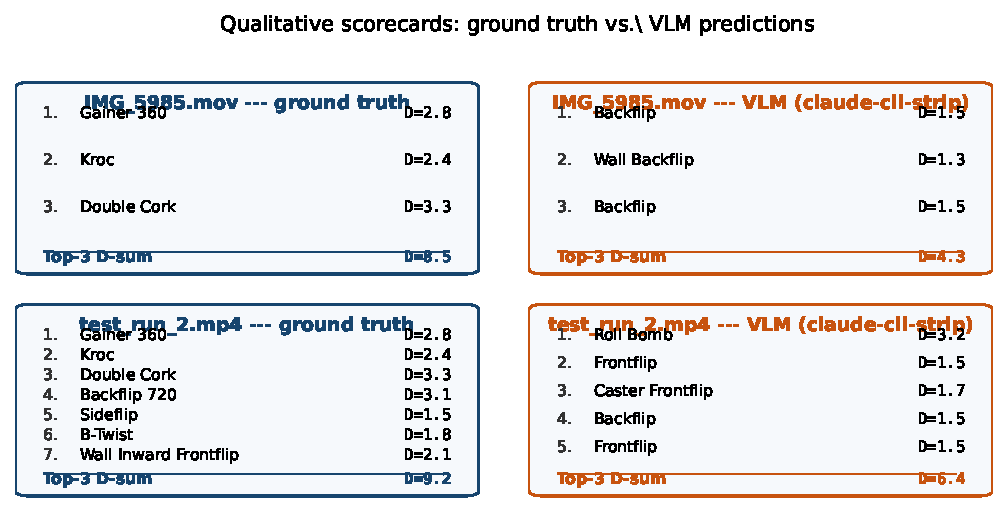
\includegraphics[width=\linewidth]{figures/fig08_scorecards.pdf}
  \caption{\textbf{Qualitative scorecards} for two POOL-A runs.
  Left of each row: the ground-truth FIG trick list and top-3 D-sum.
  Right: the best-performing VLM's prediction on each segment from
  the inversion segmenter. Correct identifications, mis-calls, and
  the resulting top-3 D-sum are shown side by side. The segmenter
  consistently finds the right number of trick segments; the VLM is
  the weak link.}
  \label{fig:scorecards}
\end{figure}

\subsection{Failure Modes}
\label{sec:experiments:failures}

\begin{figure}[t]
  \centering
  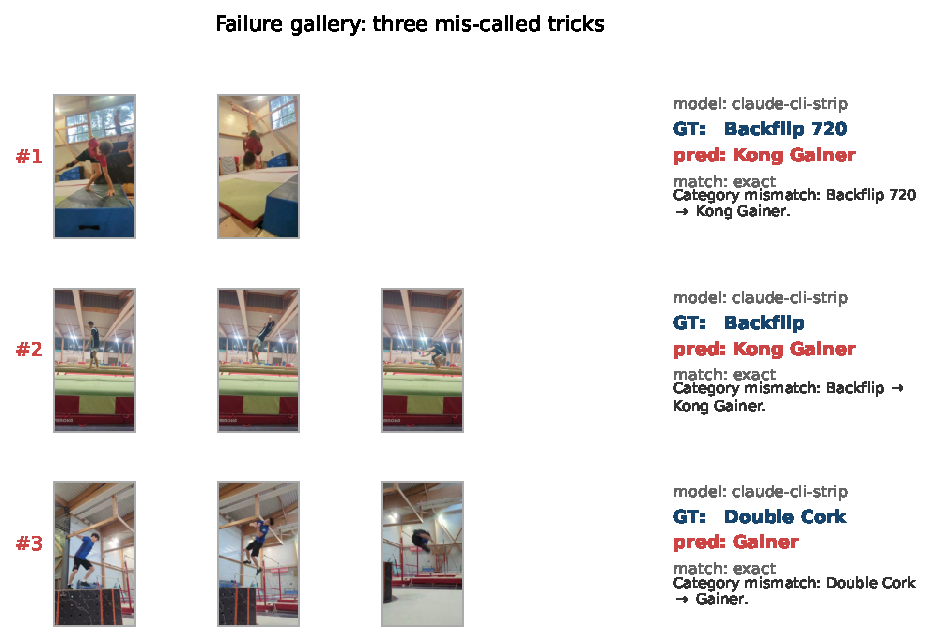
\includegraphics[width=\linewidth]{figures/fig09_failure_gallery.pdf}
  \caption{\textbf{Failure gallery.} Three mis-called clips from
  POOL-B with their ground-truth label, VLM prediction, fuzzy-matcher
  level, and a short diagnosis.}
  \label{fig:failures}
\end{figure}

Inspecting the full \texttt{results.jsonl} reveals three recurring
failure modes:

\begin{itemize}
  \setlength\itemsep{-1pt}
  \item \textbf{Twist under-counting on multi-twist tricks.} The
        models reliably recognise a backflip, but the twist count
        they return is almost always too low, mapping a Backflip 720
        to a Backflip or Backflip 360 and a Gainer 360 to a plain
        Gainer. The predicted physical attributes in the raw output
        are internally consistent with the (wrong) name, which
        suggests the models are undersampling the actual number of
        revolutions rather than guessing the name blindly.
  \item \textbf{Takeoff confusion between gainer-like and standing
        tricks.} All three models frequently substitute ``Kong
        Gainer'' or ``Gainer'' for tricks that have the same flip
        signature but a different takeoff. The distinction requires
        reading the pre-takeoff foot contact, which is the region of
        the clip with the least inverted motion and therefore the
        part the models seem to weight least.
  \item \textbf{Wall-context loss.} Wall-contact inward flips
        (Wall Inward Frontflip / Wall Inward Sideflip) are frequently
        scored as ground frontflips because the wall itself is often
        off-frame by the time the athlete inverts. The fuzzy matcher
        cannot rescue this because the VLM confidently outputs a
        ground-category name.
\end{itemize}

All three of these are \emph{physics} errors: a hypothetical system
that combined the VLM noun with a reliable 3D-pose twist counter and
an apparatus-context detector would, in principle, fix each of them
without changing the VLM component. Sec.~\ref{sec:discussion}
discusses what we think the minimum next step is.

\subsection{Ablations and Observations}
\label{sec:experiments:ablations}

\paragraph{Frames vs.\ strip for Claude.}
An initial attempt at the Claude CLI used eight separate frame files
and asked the model to read them in order with its \texttt{Read}
tool. Across the same POOL-B clips, this configuration produced
confident but fabricated narratives: Claude would describe an
athlete catching a bar, climbing a wall, or walking through an
obstacle sequence that did not exist in the 1--2-second clip. We
attribute this to the loss of temporal continuity when each frame
is processed as a separate tool call. Moving to a single composite
strip image with the frames labeled 1--8 removed the hallucinations,
which is why the strip encoding is our default. We nevertheless
\emph{still} find the headline accuracy low in strip mode, so the
fix is necessary but not sufficient.

\paragraph{Interactive vs.\ headless for VLMs.}
In an earlier manual test, a human operator loaded the same frame
strips for \texttt{IMG\_5985.mov} into Claude Code in interactive
mode and asked ``what trick is this''. Claude correctly identified
the Gainer, the Kroc, and the Double Cork. In the present paper
Claude-CLI-strip in headless \texttt{-p} mode on the same clips
returns different, lower-quality answers. We do not have a clean
explanation for this gap beyond the plausible candidates of
(i)~different default temperature, (ii)~the absence of
conversational scaffolding in headless mode,
(iii)~tool-call accounting, or (iv)~sampling variance. We
document this \emph{automation gap} as a finding that a practitioner
wiring a frontier VLM into a batch pipeline should expect to
encounter. Multi-sample voting, a higher-quality system prompt, and
an interactive-mimicking agentic loop are all natural next steps
that are out of scope for this paper.

\paragraph{Gemini quota issues.}
We were unable to run a full POOL-B pass with Gemini~2.5 Pro or
Gemini~3.1 Pro~Preview during the benchmark window. Both hit
persistent HTTP~429 errors---Gemini~2.5 Pro on the free Google AI
tier (per-minute quota), Gemini~3.1 Pro~Preview on Google's shared
\texttt{cloudcode-pa.googleapis.com} backend
(\texttt{MODEL\_CAPACITY\_EXHAUSTED}, not a per-user limit). The
results in Table~\ref{tab:main_results} should therefore be read as
``frontier VLMs in a free-tier accessible configuration''; a paid
Gemini~2.5 Pro deployment or a future stable Gemini~3 release may
well tell a different story.

\paragraph{What remains solid.}
Even with weak VLM accuracy, the system's non-VLM components work
reliably. The inversion segmenter finds exactly three trick segments
on \texttt{IMG\_5985.mov} and they overlap the three real tricks
(Fig.~\ref{fig:segmentation}); the fuzzy matcher snaps every
well-formed VLM output to a FIG entry at the first cascade level;
the D-score assembler is deterministic by construction. The
weakness of the system is confined to the \emph{identification}
step, which suggests that a stronger VLM---or a VLM paired with
a physics twist counter---would lift the whole pipeline without
requiring any of the other components to change.

\section{Discussion}
\label{sec:discussion}

\paragraph{Why we still think the VLM route is correct.}
Our main results are unflattering but the broader argument of the
paper stands: a parkour trick name is a \emph{linguistic} label over
a set of physical motions, not a set of motions in itself. ``Cork''
is a word that athletes and judges agreed means ``a backflip with a
half twist on a tilted axis''. It is a compositional entry in a
shared taxonomy that VLMs have absorbed from the parkour and tricking
internet at scale. A trained video classifier has to discover that
taxonomy from a few hundred clips per family and---as we show in
Sec.~\ref{sec:journey}---consistently fails to do so on our dataset.
The finding from our benchmark is not ``VLMs don't know parkour''
but rather ``frontier VLMs know parkour nouns better than they count
parkour revolutions, and in headless automation mode they have a
tendency to answer the wrong noun anyway.''

\paragraph{The automation gap.}
The most surprising and practically actionable result of the paper
is the gap between interactive and headless behaviour of the same
VLM on the same clips. In the absence of a clean explanation we
cannot, in good conscience, claim that a one-shot headless pipeline
is a solved problem. But we can name the gap and invite follow-up
work. Hypotheses worth testing in future work include:
\begin{itemize}
  \setlength\itemsep{-1pt}
  \item Interactive chat sessions carry a richer system prompt that
        includes instructions to reason carefully before answering.
  \item Headless mode's default temperature produces more
        confident-but-wrong samples than a human user would see,
        because the human would retry or ask a follow-up question.
  \item Tool-call accounting: interactive mode may allow the model
        more internal scratchpad reasoning before producing a final
        answer.
  \item Sampling variance: with 13 clips and one shot per model,
        every run is a draw from a noisy distribution.
\end{itemize}
Each of these is a small empirical study that would sharpen the
present result. We explicitly position this paper as a baseline that
the next wave of experiments can improve on.

\paragraph{The matcher is load-bearing, even when the predictions are
wrong.}
Table~\ref{tab:matcher_levels} shows that whenever a VLM returns a
trick name, the fuzzy matcher snaps it to a FIG entry with high
confidence, usually at the L1 exact level. The cascade therefore
carries very little of the load on our benchmark---the VLMs happen
to emit in-table names, even when those names are wrong. We still
believe the cascade is a load-bearing piece of the system because
(i)~it is the component that makes the VLM interface deterministic
and auditable, and (ii)~we saw informal VLM queries produce names
like ``back double full'', ``cork screw'', and ``krok'' that do need
the L2--L4 levels. A longer benchmark would likely exercise the
full cascade more thoroughly.

\paragraph{What the failure gallery tells us about the next system.}
All three of the recurring errors documented in
Sec.~\ref{sec:experiments:failures}---twist under-counting, takeoff
confusion, wall-context loss---are \emph{physics} errors that a
classical pose-tracking pipeline would be well-positioned to fix if
its input were reliable. That observation suggests a very concrete
next architecture: use the VLM only for the trick \emph{noun} (what
family of move is this), and delegate the \emph{attributes} (flip
count, twist count, direction, takeoff) to a deterministic physics
component driven by a 3D pose estimator fine-tuned on acrobatic
motion. The FIG table is compositional, so two small, well-aligned
signals would cover the whole space without the VLM having to count
twists at all. We leave this hybrid to future work; the present
paper argues only that the noun-only VLM path is the right starting
point and that the physics path remains necessary.

\paragraph{Cost, latency, deployability.}
Across the three configurations we benchmarked, a single trick
identification costs tens of seconds and a few cents or nothing
at all (Claude via an existing CLI subscription). A full competition
run of eight tricks is therefore fast and cheap enough to be useful
as an advisory tool during a live event, even if the accuracy
remains low: a human judge could in principle be shown the full
D-score card and correct only the entries the system flagged as
uncertain. None of our experiments tested this interactive
judge-assistance mode, but the system's text-level interfaces
(FIG name + match level + reasoning in every output) make it
straightforward to plug in.

\paragraph{Ethical note.}
We explicitly do not recommend using the raw \sys{} scorecard as a
substitute for a human judge's final score. The current accuracy is
too low, and the system is deliberately transparent about which
decisions it was confident in and which it was not. We hope the
fact that \sys{} is open-source and fully auditable---every
prediction records its model version, prompt hash, match level,
and raw text---means that any follow-up deployment will be on terms
a parkour federation can inspect before trusting.

\section{Limitations}
\label{sec:limitations}

\sys{} has several concrete limitations, some of which are artefacts of
this study and some of which are structural.

\paragraph{Small evaluation set.}
POOL-A contains four competition runs and POOL-B contains tens of
single-trick segments. This is a case study, not a statistically powered
benchmark. We report per-clip numbers rather than only aggregate means so
readers can form their own picture, and we release the clips and labels
so the community can extend the set. A larger, multi-annotator benchmark
is the natural next paper.

\paragraph{Single-annotator ground truth.}
All labels were assigned by the author. For tricks with clear visual
identity (backflip, frontflip, gainer), this is uncontroversial. For
multi-twist tricks and off-axis variants, human judges themselves
disagree, and a single annotator is insufficient. We release
\texttt{ground\_truth.csv} with a \texttt{notes} column so external
annotators can propose corrections.

\paragraph{Closed-model dependence.}
The strongest configurations in the leaderboard are closed-weight
frontier models (Gemini 2.5, Claude Sonnet 4.5). Their behaviour may
change between versions, which is a reproducibility risk. We mitigate
this by (i) always including an open-weight comparison point
(Qwen2.5-VL 72B), (ii) logging the exact model version string in every
\texttt{results.jsonl} record, and (iii) releasing the full prompt and
fuzzy matcher so the \emph{system} is reproducible even if specific
weights drift.

\paragraph{Monocular video only.}
Real competitions film from multiple synchronised angles. A
multi-camera extension of \sys{} would plausibly resolve most
off-axis and wall-context failures documented in
Sec.~\ref{sec:experiments:failures}, but is out of scope here. We
note only that the fuzzy matcher and D-score assembler are camera-count
agnostic and could be reused as-is.

\paragraph{D-score only.}
FIG judging decomposes into a D-score (difficulty, from the table of
tricks) and an E-score (execution, deductions for safety, landing
quality, and flow). \sys{} addresses only the D-score; landing quality
and flow scoring require frame-level body-pose analysis that VLMs are
currently not precise enough to provide. We explicitly position the
E-score as future work, not as a broken promise.

\paragraph{Segmentation robustness.}
The inversion segmenter assumes the athlete becomes inverted during the
aerial phase. This holds for all acrobatic and wall tricks in the FIG
2025 table, but misses low-rotation moves (swing 180, wall spins) and
is confused by crowd members who happen to bend over at the wrong
moment. A context-aware segmenter driven by an additional VLM call is a
natural next step.

\section{Conclusion}
\label{sec:conclusion}

We presented \sys{}, an open-source pipeline that takes a monocular
parkour video and produces a FIG-compliant D-score scorecard
without a single training label. The system is deliberately built
out of components that any researcher with a laptop and an API key
can run today: YOLO-pose for tracking, an inversion signal for
segmentation, an off-the-shelf vision--language model for naming,
a five-level fuzzy matcher against the 149-entry FIG table, and a
deterministic D-score assembler. Over eighteen months we
abandoned five trained-model configurations before arriving at
this one; Sec.~\ref{sec:journey} records why each of them failed.

Our empirical contribution is a deliberately honest one. On 13
curated single-trick clips, three frontier vision--language models
(Claude Sonnet~4.5, Gemini~2.5 Flash, Qwen2.5-VL~72B) achieve low
top-1 accuracy in headless automation mode, even though the same
models correctly name the same tricks when queried interactively
through a chat interface. We have named the resulting
\emph{automation gap}, catalogued the three recurring physics
failures (twist under-counting, takeoff confusion, wall-context
loss), and shown that the non-VLM components of the pipeline---the
segmenter, the fuzzy matcher, the D-score assembler---continue to
work independently of which VLM is plugged in.

We believe the parkour judging problem decomposes cleanly into a
\emph{naming} problem and a \emph{physics} problem. The present
paper argues that VLMs are already on the right side of the naming
problem but not yet reliable in automation, and that a hybrid
pipeline that pairs a VLM noun with a physics twist counter is the
natural next step. We release the full system, prompts, ground-truth
labels, raw \texttt{results.jsonl}, and figure-generation scripts at
\url{https://github.com/AirKyzzZ/pkvision} and actively invite
corrections to the FIG trick table, external labels, and experiments
that push any component of the pipeline forward.

Our immediate next steps are (i)~a multi-annotator, multi-shot
benchmark drawn from public FIG competition footage, with temperature
zero and multi-vote aggregation to separate the automation gap from
pure sampling noise; (ii)~a VLM-plus-physics hybrid that delegates
twist counting to a fine-tuned 3D pose module trained on acrobatic
data; and (iii)~integration with a live-event web interface so the
system can act as an advisory tool during FIG qualifiers, with every
decision auditable by the judges on the panel.


{
    \small
    \bibliographystyle{ieeenat_fullname}
    \bibliography{references}
}

\appendix
\section{Appendix: Full Prompt and Per-Run D-Score Sheets}
\label{sec:appendix}

\TODO{Appendix --- drafted in Phase 5.}


\end{document}
